%*******************************************************************************
%****************************** Second Chapter *********************************
%*******************************************************************************

\chapter{Theoretical Overview}
\label{ch:theory}

\ifpdf
    \graphicspath{{Chapter2/Figs/Raster/}{Chapter2/Figs/PDF/}{Chapter2/Figs/}}
\else
    \graphicspath{{Chapter2/Figs/Vector/}{Chapter2/Figs/}}
\fi


%********************************** % First Section  *************************************

The Standard Model (SM), proposed in the 1960s, has long been the most prominent and
successful description of fundamental particles and their interactions at the
energies currently experimentally accessible. Its power has been proven with the 
theoretical prediction of particles such as the charm and top quarks, and the W
and Z bosons, prior to their experimental observation. Furthermore, precision 
electroweak measurements have shown impressive levels of  agreement with SM
predictions \cite{ALEPH:2010aa}.

However, despite its great success, it is known to be valid only for low 
energies, and is missing significant details of both experimentally 
observed and theoretically predicted physical phenomena. As such, extensions to
the SM have been extensively studied, assuming the SM to be the low-energy 
regime of some greater theory. One such strongly theoretically motivated
extension to the SM is Supersymmetry (SUSY).

This chapter first outlines the SM model, including its particle content and basic 
mechanisms, before describing its shortcomings - the theoretical 
motivation for Beyond the Standard Model (BSM) theories. SUSY will then be 
introduced, before describing its simplest incarnations, along with a discussion
of the specific models and frameworks used for interpretation within this
analysis.

\section{The Standard Model}
\label{sec:theory_current}

The Standard Model is a renormalisable Quantum Field Theory describing
fundamental matter particles and their interactions via the strong,
weak and electromagnetic forces. It was collaboratively developed throughout the
1960s \cite
{Glashow1961579,PhysRevLett.19.1264,Salam:1968rm,PhysRevLett.30.1346,PhysRevLett.30.1343}, with its current Lagrangian
based formalism being finalised in the mid-1970s \cite{martinAndShaw}.

Requiring local gauge invariance of the SM Lagrangian, $\mathcal{L}_{SM}$,
under
transformations generated by universal space-time symmetry groups,
interactions can be described via conserved quantities. The $SU(3)$ group
describes strong force interactions through colour charge, and $SU(2)$ and $U(1)$ to
describe electroweak interactions through weak isospin and hypercharge respectively.

% The requirement that $\mathcal{L}_{SM}$ be invariant under local gauge
% transformations dictates the structure, and crucially the particle content of
% the SM.

Matter particles are described by spin 1/2 fermions, summarised in
table~\ref{tab:sm_fermions}, divided into the six quarks
and six leptons. The quarks, are arrange into three generations: the up($u$) and
down($d$), the charm($c$) and strange($s$), and the top($t$) and bottom($b$),
each couplet carrying
individual electric charges of +2/3 and -1/2 respectively. The quarks also carry
colour charge, where combinations of quarks form colour-neutral composite
hadron particles which are observed in nature.

% matter particles are described by spin 1/2 fermions, divided into the six quarks and six 
% leptons. the quarks are arranged in three generations, the up and down, the charm
% and strange, and the top and bottom, carrying electric charges of +2/3 and -1/2 
% respectively. the quarks also carry a colour charge, where only colour-neutral 
% composite hadron particles, combinations of quarks, are seen in nature.

The leptons are similarly arranged into three generations, constructed from
$SU(2)$
doublets of weak isospin, $(\nu_L, l)_L$, of left-handed chiral states, and
singlets, $l_R$, of right-handed chiral states, where $l$ represents either the
electron ($e$), muon ($\mu$) or tau ($\tau$), each carrying a -1 electrical
charge, and $\nu_L$ being their corresponding electrically neutral neutrinos.

% the leptons again are arrange in three generations, constructed from SU(2) 
% doublets of weak isospin (neutrino L, l)L of left-handed states, and singlets of
% lR right-handed states, where l represents the electron, muon and tau, each with
% -1 electric charge. with vl being their corresponding electrically neutral neutrinos.

\begin{table}[h!]
  \caption{The fermion particle content of the Standard Model \cite{Agashe:2014kda}.\label{tab:sm_fermions}}
  \centering
  \small
  \begin{tabular}{ lcccc }
    \hline
    \hline
    Name        & Type & Spin & Charge (e) & Mass \\
    \hline
    Electron ($e$)              & Lepton    & 1/2    & -1     & 0.511 MeV  \\
    Electron Neutrino ($\mu_{e}$)& Lepton   & 1/2    & 0      & -  \\
    Muon ($\mu$)                & Lepton    & 1/2    & -1     & 105.658 MeV  \\
    Muon Neutrino ($\nu_{\mu}$) & Lepton    & 1/2    & 0      & - \\
    Tau ($\tau$)                & Lepton    & 1/2    & -1     & 1.776 GeV  \\
    Tau Neutrino ($\nu_{\tau}$) & Lepton    & 1/2    & 0      & - \\
    Up ($u$)                    & Quark     & 1/2    & +2/3   & $2.3^{+0.7}_
    {-0.5}$ MeV \\
    Down ($d$)                  & Quark     & 1/2    & -1/3   & $4.8^{+0.5}_
    {-0.3}$ MeV \\
    Charm ($c$)                 & Quark     & 1/2    & +2/3   & $1.275 \pm
    0.025$ GeV \\
    Strange ($s$)               & Quark     & 1/2    & -1/3   & $95 \pm 5$ MeV\\
    Top ($t$)                   & Quark     & 1/2    & +2/3   & $173.21 \pm 0.51
    \pm 0.71$ GeV \\
    Bottom ($b$)                & Quark     & 1/2    & -1/3   & $4.66 \pm 0.03$
    GeV \\
    \hline
    \hline
  \end{tabular}
\end{table}

\begin{table}[h!]
  \caption{The boson particle content of the Standard Model \cite{Agashe:2014kda}.\label{tab:sm_bosons}}
  \centering
  \small
  \begin{tabular}{ lcccc }
    \hline
    \hline
    Name                            & Force Carried & Spin & Charge (e) & Mass \\
    \hline
    W Boson ($W$)     & Weak        & 1    & $\pm 1$  & $80.385 \pm 0.015$ GeV \\
    Z Boson ($Z$)     & Weak        & 1    & 0        & $91.188 \pm 0.002$ GeV \\
    Gluon ($g$)       & Strong      & 1/2  & 0        & - \\
    Photon ($\gamma$) & Electromagentism   & 0  & 0   & - ( or < $1\times10^
    {-18}$
    eV)\\
    Higgs Boson ($H$) & -           & 0    & 0        & $125.7 \pm 0.4$ GeV \\
    \hline
    \hline
  \end{tabular}
\end{table}

Interactions between the fermions are mediated by spin-1 bosons, shown in
table~\ref{tab:sm_bosons}. The strong 
force, $SU(3)$, is represented by eight electrically neutral, massless gluons 
($g$), each carrying a colour charge. The electroweak force, $SU(2)\times U(1)$
is
mediated by the electrically neutral, massless photon ($\gamma$), the massive,
neutral $Z^0$, and the massive, electrically charged $W^{\pm}$ bosons.

Following the enforcement of local gauge invariance after an
$SU(2)\times U (1)$ transformation,
the bosonic mediator of the $U(1)$ symmetry, the $\gamma$, remains massless as
expected, however so do the $W^{\pm}$ and $Z^0$, in disagreement with their
experimentally observed masses. To remedy this, the $SU(2)\times U(1)$ symmetry
undergoes Electroweak Symmetry Breaking (EWSB) via the Higgs Mechanism
\cite{PhysRevLett.13.321,PhysRevLett.13.508,PhysRevLett.13.585}, 
leading to the Higgs boson, $H^0$, a massive, electrically neutral, spin-0
scalar particle, thereby completing the formalism of the Standard Model.

% finally, the electroweak sector, SU(2)xU(1) is spontaneously broken by the 
% massive, neutral, spin-0 scalar boson H0, allowing for massive particles to 
% attain mass. couples in proportion to mass.

% \emph{does it give masses to every massive particle, or just W/Z and this 
% propogates mass?}

\subsection{Failings of the Standard Model}

While the Standard Model has provided many accurate predictions and descriptions
which have been extensively experimentally verified \cite{Baak:2014ora}, the
theory is considered incomplete due to gaps in its description of the Universe.

The SM provides a QFT description of how the strong, weak and electromagnetic
forces work on a quantum level, however it fails to include any description of
the final fundamental force, gravity. A quantum description of gravity has long
been sought after by particle theorists, in particular to provide an explanation
for its relative weakness at the Electroweak scale with respect to the other
fundamental forces.

Following the Big Bang it is believed matter and anti-matter were created in
equal amounts, however given that we exist in a matter dominated universe there
must exist some physical process by which an asymmetry came to be between the
two types of matter - the so-called `Baryogenesis' process. This could
be described by violation of the Charge-Parity (CP) symmetry,
however the amount of CP violation described by the Standard Model
does not appear to be significant enough to achieve this REF.

In the SM, following the local gauge invariance requirement of the electroweak
sector, $SU(2)\times U(1)$, the $SU(2)$ doublets contain
massless neutrino particles. However, experimental observations of neutrino
oscillation between their various flavours indicate them to have finite mass
\cite{PhysRevLett.81.1562,PhysRevLett.89.011302}, and can
therefore mix between different mass eigenstates. This is only described
by extending the Standard Model to include neutrino mixing, defined by the
PMNS matrix \cite{Altarelli:2002hx}.

Furthermore, and of particular relevance to the work in this this thesis, are
the Hierarchy Problem and the existence of Dark Matter.

\subsubsection{The Hierarchy Problem}

% When calculating beyond tree-level diagram contributions to the Higgs mass,
% $m_h$, divergent terms arise which make the mass increase up to values in
% strong disagreement with the experimentally observed $m_h \approx 125~\gev$ REF.

Particles couple to the Higgs field according to the Yukawa couplings,
$\lambda_f$,
proportional to the mass of the particle. For fermions, the Lagrangian
interaction term is
% 
\begin{equation}
\mathcal{L}_\text{Yukawa} = - \lambda_f \bar{\Psi}H\Psi,
\end{equation}
% 
where $\Psi$ is a spin-1/2 Dirac field, and $H$ the Higgs field. Higgs mass
corrections due to beyond tree-level interactions with fermion
fields (shown in figure~\ref{fig:quantum_higgs_fermion_loop}) can be shown to
result in
% 
\begin{equation}
% \Delta m_H^2 = -\frac{|\lambda_f|^2}{8\pi^2} [\Lambda_{\text{cut}}^2 + \ldots]
\Delta m_H^2 \propto -|\lambda_f|^2 \Lambda_{\text{cut}}^2,
\label{eq:higgs_corr_hierarchy}
\end{equation}
% 
where $\Lambda_{\text{cut}}$ is the cut-off energy scale, up to which the SM is
valid, typically taken to be the Planck scale. This therefore leads to a
quadratically
divergent correction to $m_H$. Such corrections cause significant tension
between the theoretically allowed value of $m_H$ and the experimentally
measured value, $m_H \simeq 125$~\gev \cite{PhysRevLett.114.191803},
requiring significant `fine-tuning' to bring the two into agreement. This
disagreement is known as the Hierarchy Problem.

\begin{figure}[t]
\centering
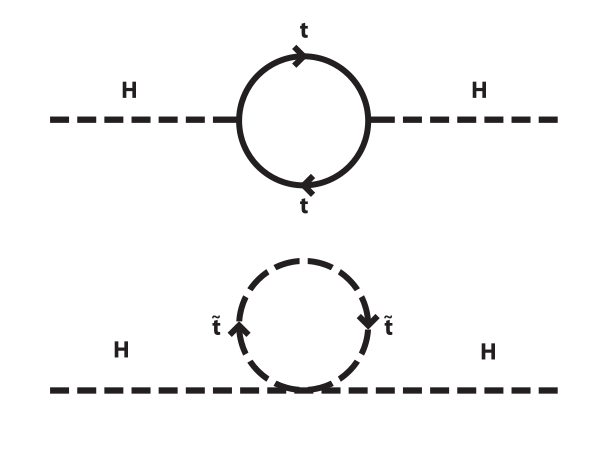
\includegraphics[width=0.47\textwidth,trim=0 250 0 0, clip=true]
{Figs/feynman/600px-Hqmc-vector.png}
\caption{Quantum self-corrections to the Higgs mass from a fermionic top quark
loop.}
\label{fig:quantum_higgs_fermion_loop}
\end{figure}

\subsubsection{Dark Matter}
Significant amounts of Dark Matter (DM) have been indirectly observed
through the study of galaxy rotation curves and
gravitational lensing techniques\cite{Corbelli15012000,0004-637X-744-2-159}. For
such a large relative abundance to be present, DM must be massive and weakly
interacting. No candidate particle exists in the SM to describe such
matter.

%********************************** % Second Section  *************************************
\section{Supersymmetry}  %Section - 1.2
\label{sec:theory_overview}
At its core, Supersymmetry is a new space-time symmetry
between fermions and bosons \cite{ref:SUSY-1,ref:SUSY0,ref:SUSY1,ref:SUSY2,ref:SUSY3,ref:SUSY4}.
An operator of SUSY acting on a fermion
(resp. boson) state acts to change the spin by a 1/2, producing a super-partner
boson (resp. fermion) state, maintaining electric charge, colour charge and weak
isospin. A theory invariant under such transformations is said to be
supersymmetric.

As a consequence of this new symmetry, SUSY introduces a rich phenomenology of
new particles (sparticles). The simplest implementation of SUSY is the
Minimally
Supersymmetryic Standard Model (MSSM) \cite{Martin:1997ns} - a so-called
`complete' model, containing more than 100 free-parameters representing
sparticle masses, phases and mixing angles \cite{Dimopoulos:1995ju}.
Within the MSSM, the SU(2) doublets and singlets, $(\nu_L, l)_L$ and $l_R$,
have super-partners $(\tilde{\nu}_L, \tilde{l})_L$ and $\tilde{l}_R$. Similarly
for SU(3), $(q, q')_L$ and $q_R$,
have super-partners $(\tilde{q}_L, \tilde{q}')_L$ and $\tilde{q}'_R$. The
spin-1 SM gauge bosons have spin-1/2 gaugino partners, the gluino, winos and
bino, $\tilde{g}$, $\tilde{W}^{\pm}$, $\tilde{W}^0$, $\tilde{B}^0$.
The Higgs sector is extended to include
two Higgs-doublets giving five mass-eigenstates, $h^0$, $H^0$, $A^0$ and
$H^{\pm}$. Finally, the gauginos and the neutral higgsinos mix to give the
neutralinos, $\tilde{\chi}^0_{i=1-4}$, and the winos and charged higgsinos mix
to give the charginos, $\tilde{\chi}^{\pm}_{i=1-2}$.

\begin{table}[h!]
  \caption{The particle content of the Minimally Supersymmetric Standard
  Model. Note that there are now two Higgs doublets present.\label{tab:susy_particles}}
  \centering
  \small
  % \setlength\extrarowheight{5pt}
  \begin{tabular}{ lccc }
    \hline
    \hline
    Sparticle         & Partner  & Spin & Charge (e) \\
    \hline
    $\chiz_0, \chiz_1, \chiz_2, \chiz_3$ & $\gamma, Z, H^0, h^0$ & 1/2 & 0 \\  
    $\chipm_0, \chipm_1$ & $W^{\pm}, H^{\pm}$ & 1/2 & $\pm1$ \\
    
    $\widetilde{e_{\bar{L}}}, \widetilde{e_{\bar{R}}},
    \widetilde{\nu_e},
    \widetilde{\mu_{\bar{L}}},$ &\multirow{2}{*}{$e, \nu_{e}, \mu, \nu_{\mu}, \nu_{\tau}$}&\multirow{2}{*}{1} & \multirow{2}{*}{$\pm 1$, 0} \\
    $ \widetilde{\mu_{\bar{R}}}, \widetilde{\nu_{\mu}},
    \widetilde{\nu_{\tau}}$ &&&\\
    
    $\widetilde{\tau}_L, \widetilde{\tau}_R$ & $\tau$ & 1  & $\pm 1$ \\
    

    $\widetilde{u_L}, \widetilde{u_R}, \widetilde{d_L},
    \widetilde {d_R},$& \multirow{2}{*}{$u, d, s, c$} & \multirow{2}{*}{1} & \multirow{2}{*}{$\pm 1/3, \pm 2/3$} \\
    $\widetilde{s_L}, \widetilde{s_R}, \widetilde{c_L}, \widetilde{c_R}$ &&& \\
    $\widetilde{b_L}, \widetilde{b_R}$ & b & 1 & $\pm 1/3, \pm 2/3$ \\
    $\widetilde{t_L}, \widetilde{t_R}$ & t & 1 & $\pm 1/3, \pm 2/3$ \\
    $\widetilde{g}$ & g & 1/2 & 0 \\
    \hline
    \hline
  \end{tabular}
\end{table}

Given the lack of experimental evidence for SUSY, sparticles must
have higher masses than their SM partners, implying that Supersymmetry is not
an exact symmetry and must be broken by some mechanism, of which many
exist \cite{ref:hierarchy1,ref:hierarchy2}.



\subsection{Why SUSY?}
The Supersymmetric extension to the SM provides solutions to many of the
original theory's issues, for example the predicted unification of the running
gauge couplings at higher energy scales. Arguably two of the most important
solutions are described in the following sections.

\subsubsection{Hierarchy Problem}
While in the SM the Higgs gains corrections to its mass from fermion-loop
induced self-interactions, the presence of bosonic super-partners to these
fermions in a SUSY model provides additional diagrams (figure~\ref{fig:quantum_higgs_sboson_loop}),
which contribute oppositely signed terms,
% 
\begin{equation}
% \Delta m_H^2 = 2 \times \frac{\lambda_S}{16\pi^2}[\Lambda_{\text{cut}}^2 +\ldots]
\Delta m_H^2 \propto + \lambda_S \Lambda_{\text{cut}}^2 ,
\end{equation}
% 
where $\lambda_S$ is the bosonic super-partner's Yukawa coupling. The introduction
of these super-partners, and therefore their additional corrective terms,
provides an elegant solution to the hierarchy problem, where quadratic
divergences to $m_H$ are effectively cancelled by sparticle loop contributions.

\begin{figure}[ht!]
\centering
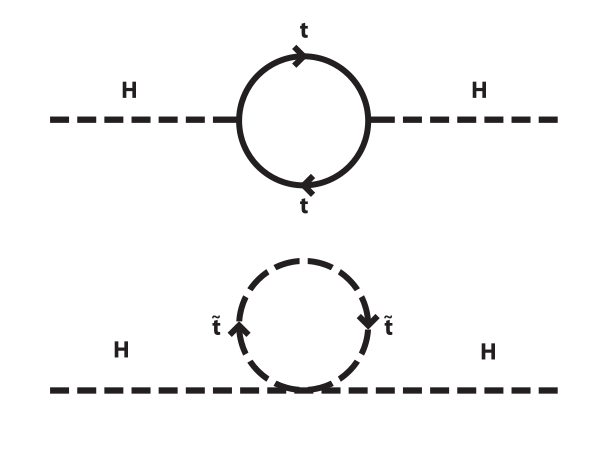
\includegraphics[width=0.47\textwidth,trim=0 0 0 250, clip=true]
{Figs/feynman/600px-Hqmc-vector.png}
\caption{Quantum self-corrections to the Higgs mass from a bosonic stop
loop.}
\label{fig:quantum_higgs_sboson_loop}
\end{figure}

\subsubsection{Dark Matter}
In many supersymmetric theories, a new conserved quantum number $R_P$
is introduced in order to conserve lepton and baryon number
\cite{Farrar1978575}, defined as
% 
\begin{equation}
R_P = (-1)^{3B+L+2s} \Bigg( =
\begin{array}{l} 
+1 \text{ for SM particles}\\ -1 \text{ for SUSY particles}
\end{array}\Bigg) ,
\end{equation}
% 
where $B$ is Baryon number, $L$ is Lepton number and $s$ is spin. SM particles
have $R_P = +1$, whereas SUSY particles have $R_P = -1$. $R_P$ is a
multiplicative quantum number, therefore sparticles
can only be pair-produced. The subsequent sparticle decay will therefore consist
of a cascade-type decay, with each sparticle decaying to a final state
containing a lighter, kinematically accessible sparticle and a SM particle.
This process will continue until the lightest supersymmetric particle (LSP) is
reached, which is therefore stable. Within R-Parity conserving models in which
the \chiz is the LSP, this particle is able to provide a stable, weakly
interacting dark matter candidate \cite{Jungman:1995df}.

% \emph{WHAT IS ELECTROWEAK BARYOGENESIS?}

\subsection{Experimental Consequences}
In order for SUSY to provide an adequate solution to the hierarchy problem,
sparticle masses are required to be around the \tev scale
\cite{ref:barbierinsusy,ref:hierarchy1,ref:hierarchy2}. This fact, coupled
with strong experimental bounds on constrained models and the discovery of
the Higgs in a compatible mass-region of the MSSM, have led interest
towards `Natural' SUSY models. Such models negate the limits imposed by
experimental constraints by assuming the first and second generation squarks to
be very heavy, while the third generation be around 1 \tev in order to solve
the hierarchy problem without significant fine-tuning
\cite{Carena:2008rt, Papucci:2011wy}.

\subsection{Simplified Model Spectra}
While `complete' supersymmetric models offer a full description of all
aspects of a given theory (e.g. mass spectra and mixing angles), the large
number of free parameters becomes unmanageable for interpretations
of experimental observations. Even in models such as the
Constrained-MSSM (CMSSM) with 5 free parameters
\cite{Kane:1993td, Ellis:2002rp}, the interpretation phase-space remains vast.

In an effort to make interpretations of experimental data simpler for
experimentalists, while remaining universally of use to theorists,
Simplified Model Spectra (SMS) were developed
\cite{PhysRevD.79.075020,Alves:2011wf}.
SMS consist of simplified
decay scenarios which can later be reinterpreted within complete models.
Typically SMS consist of either squark or gluino pair-production, with a
subsequent decay to a given final state with a 100\% branching fraction.
A crucial consequence of these models is to effectively move
experimental searches away from `model-specific' interpretations and
towards more `signature-specific' interpretations \cite{PhysRevD.88.052017}.

SMS generally contain only two free parameters, normally the mass of a
produced mother particle, $m_{\text{mother}}$, and the mass of the LSP,
$m_{LSP}$. Therefore interpretations can be made over a simple 2-dimensional
parameter space, making for trivial experimental comparisons.

SMS prove to be an excellent tool for the interpretation of results
within the bounds of naturalness. Many SMS consider third generation
squark production, allowing for direct limits to be placed on the dominant
decays of stop and sbottom squarks.

\subsection{Mass-degeneracy in the stop sector}
SUSY models with particle mass hierarchies spanning a small mass range are said to be
`compressed'. When considered in terms of a simplified model scenario, this
implies the pair-produced mother sparticle is close in mass to that of the LSP.
The
smaller the mass difference, \deltam ($= m_{mother} - m_{LSP}$), the greater the
experimental challenge, as visible
decay products become softer and typically out of analysis acceptance.

In general, decay channels of the $\tilde{t}$ are dominated by
$\sTop\ra b\chipm$ and
$\sTop\ra t\chiz$. However, when \deltam < W-boson
mass and a present W would become off-shell, $\tilde{t}$ decay branching
fractions
become
dominated by the two-body decay $\sTop\ra c\chiz$, and the four-body decay
$\sTop\ra bf\bar{f}'\chiz$ \cite{Boehm:1999tr}. In this region, these two decay
channels can provide a dark-matter relic density consistent with cosmological
observations (e.g. from WMAP \cite{Spergel:2003cb}), where annihilation cross
sections
are mediated by co-annihilation with the light stop proposed by naturalness
\cite{Balazs:2004bu,Martin:2007gf}.

This analysis will therefore focus on the two $\tilde{t}$ decays, relevant in
this highly-compressed region of SUSY phase space, namely \texttt{T2cc}
(\Ttwocc) and \texttt{T2degen} (\Ttwodegen), shown in
figure~\ref{fig:model_feynman}.

\begin{figure}[h!]
  \centering
  \hspace*{\fill}%
  \begin{subfigure}{0.35\textwidth}
    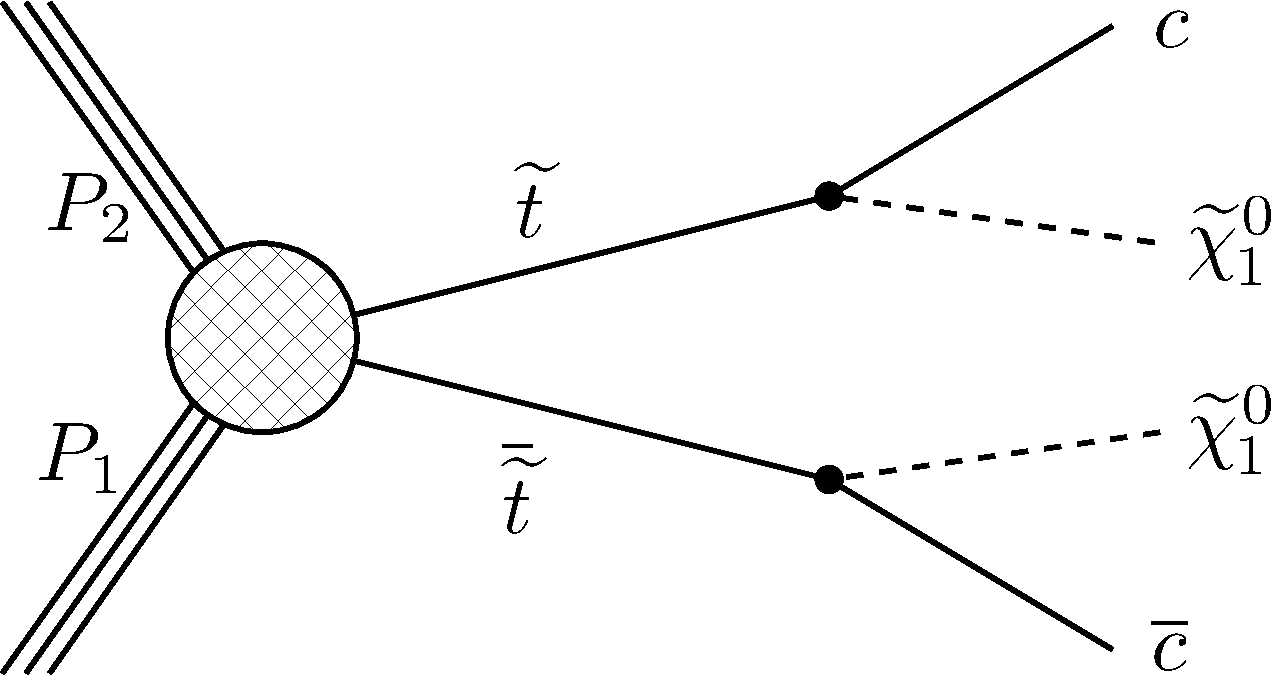
\includegraphics[width=\textwidth]{Figs/feynman/T2cc_feynman_new.pdf}
    \caption{\texttt{T2cc}}
    \label{fig:t2cc_feyn}
  \end{subfigure}
  \hfill
  \begin{subfigure}{0.35\textwidth}
    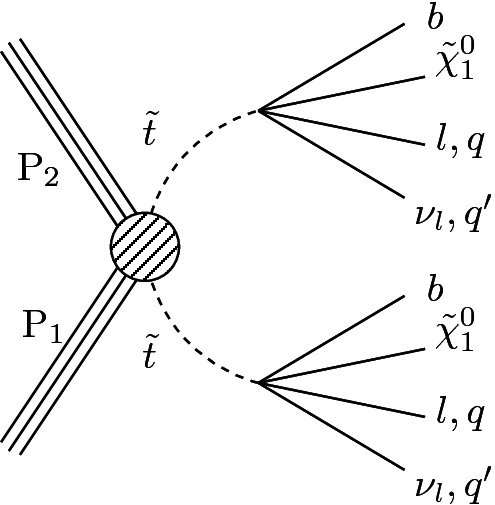
\includegraphics[width=\textwidth]{Figs/feynman/T2DegenerateStop_feyn.png}
    \caption{\texttt{T2degen}}
    \label{fig:t2degen_feyn}
  \end{subfigure}
  \hspace*{\fill}%
  \caption{Feynman diagrams of the two SMS models considered.}
  \label{fig:model_feynman}
\end{figure}

\subsubsection{Phenomenology}

\begin{figure}[h!]
  \centering
  \begin{subfigure}[b]{0.46\textwidth}
    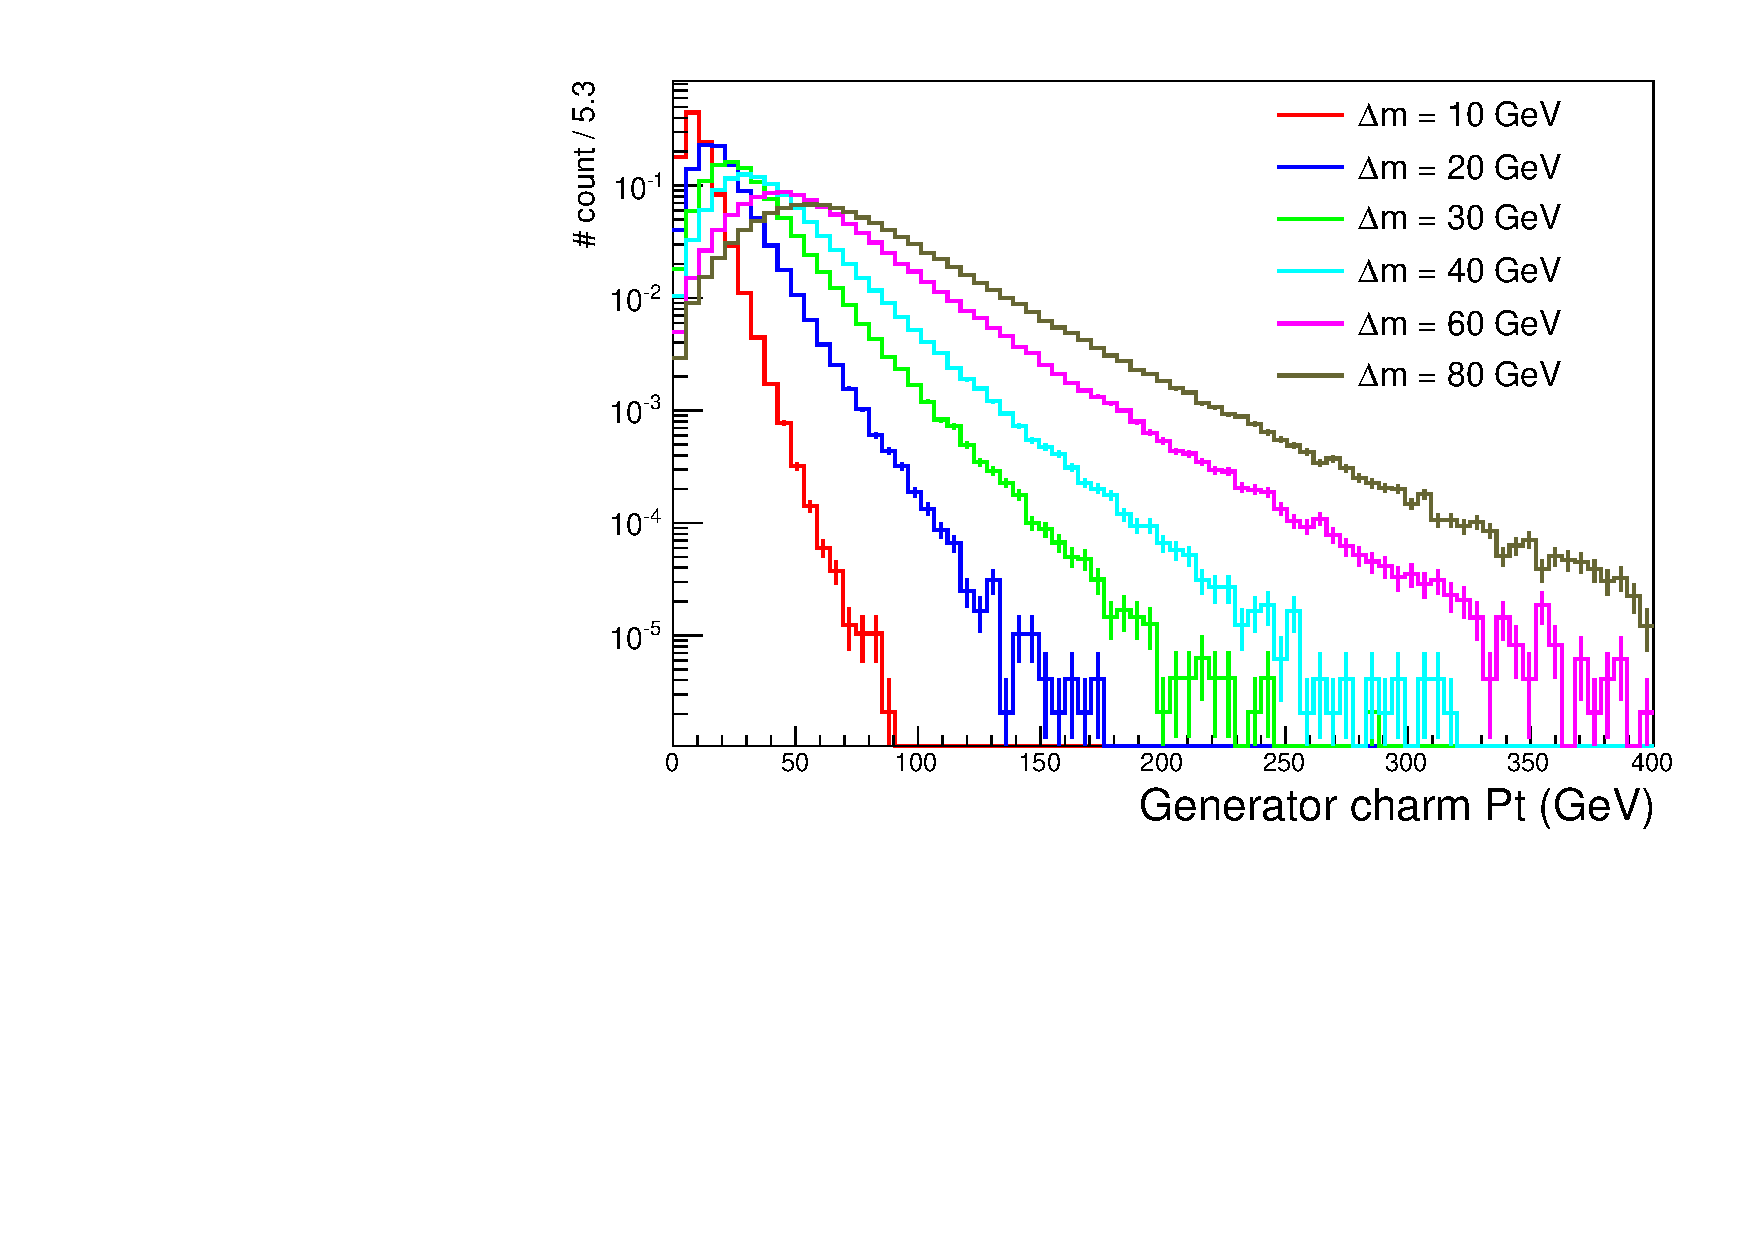
\includegraphics[width=\textwidth]{Figs/genlevel/compar_charmPt_0_0_inc_inc_T2cc_noCuts_sitv_log.pdf}
    \caption{\texttt{T2cc}}
    \label{fig:t2cc_gen_charm_pt}
  \end{subfigure}
  \begin{subfigure}[b]{0.46\textwidth}
    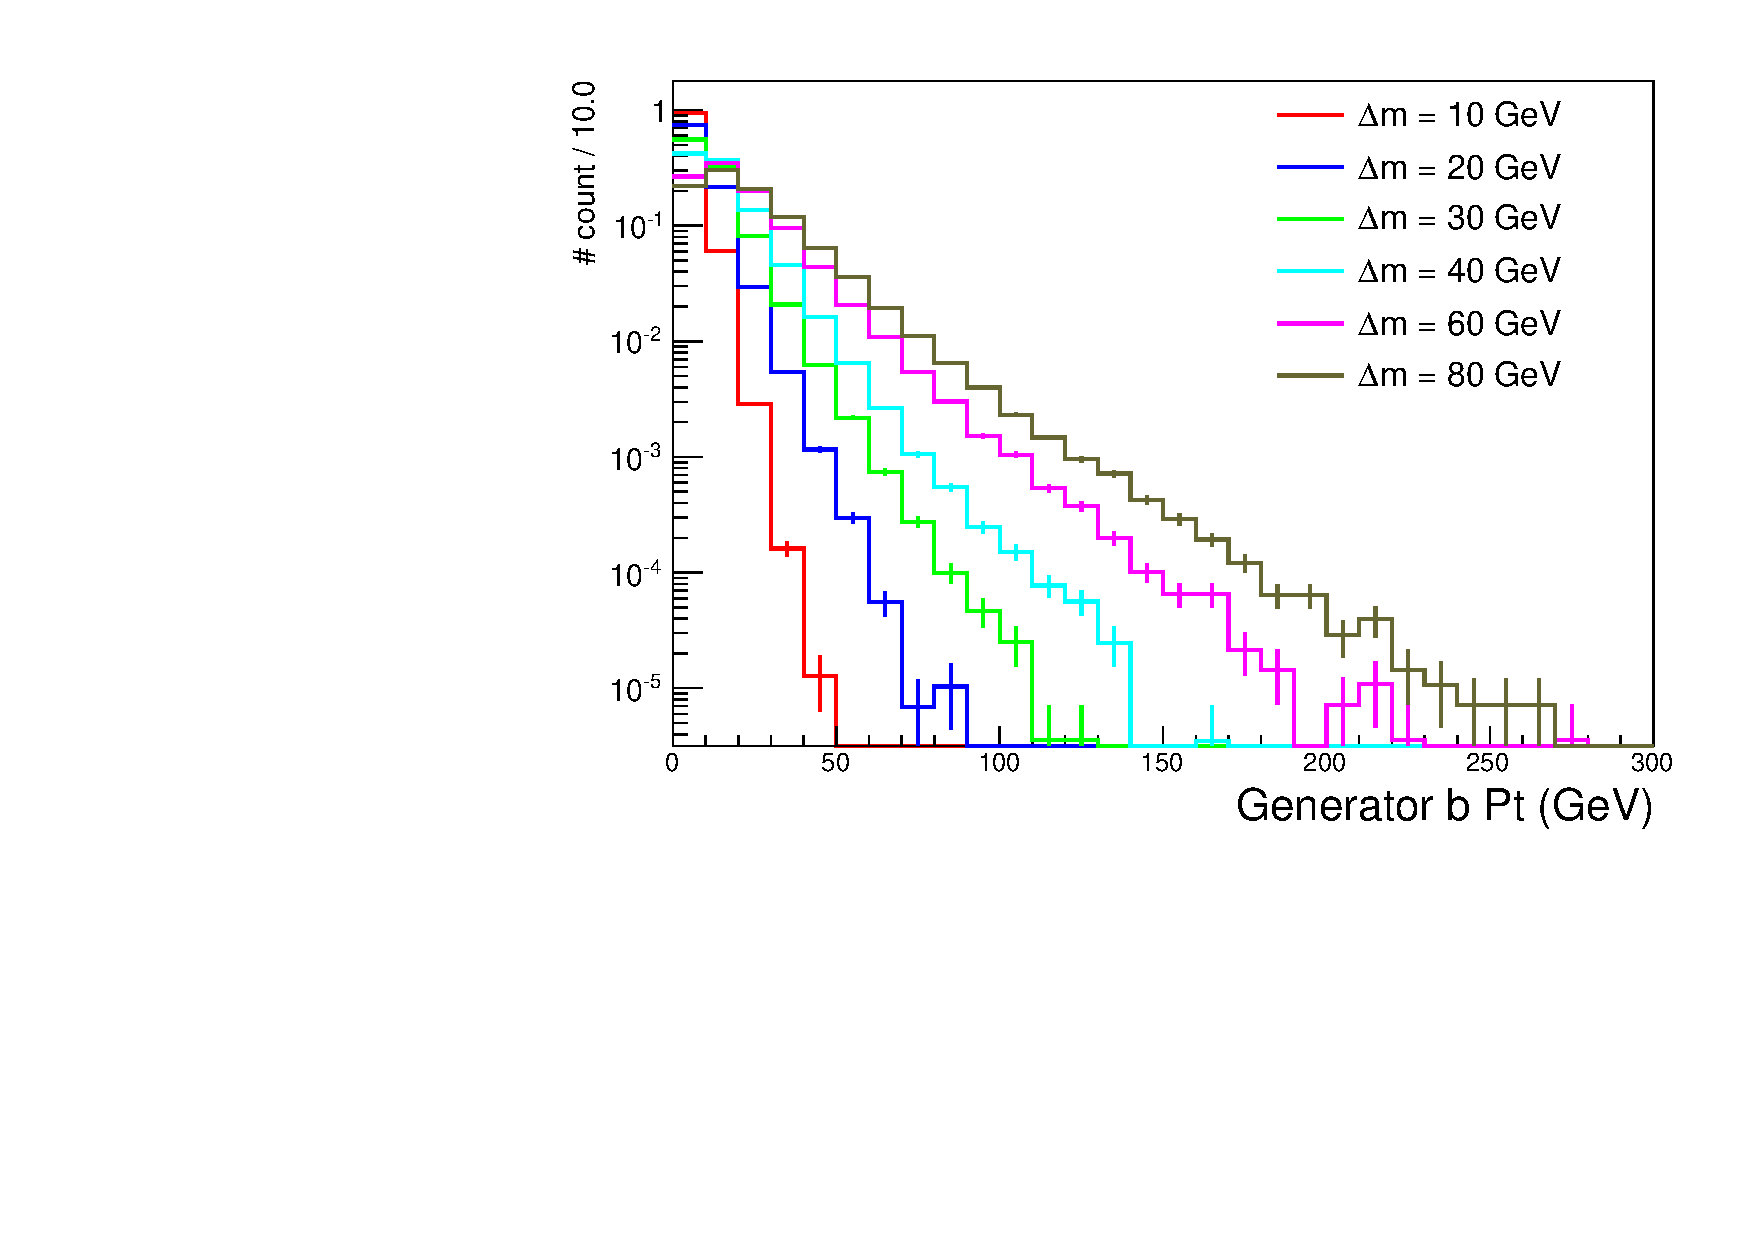
\includegraphics[width=\textwidth]{Figs/genlevel/compar_T2_4body_genBPt_0_inc_inc_T2_noCuts_sitv_log.pdf}
    \caption{\texttt{T2Degen}}
    \label{fig:t2degen_gen_b_pt}
  \end{subfigure}
  \caption{Distributions of the generator level quarks produced in the two-body
  (left) and four-body (right) decays, prior to any event selection.}
  \label{fig:gen_quark_pt}
\end{figure}

In the compressed region, characterised by small values of \deltam, decay
products of the \sTop pair have very low momenta given the small amounts of
release in the decay following the production of the \chiz. For example, 
figure~\ref{fig:t2cc_gen_charm_pt} shows the transverse momentum of the
generator level charm quark originating from the decay of the \sTop getting
smaller
with decreasing values of \deltam. Figure~\ref{fig:t2degen_gen_b_pt} shows the
same observation for the \Pt of the b quark present from the decay of the
\sTop in the 4-body decay.

The low amounts of available energy ing the small \deltam region present considerable
experimental challenges, and as such this region in the past has typically not
been considered for interpretations. The acceptance of such models in this
region is heavily reliant on initial state particles radiated from the
incoming partons, thereby boosting the decaying stops. This feature of
compressed models and it's importance to analysis sensitivity is discussed
later in chapter~\ref{ch:interpretation}.

\subsubsection{Current Experimental Limits}

\begin{figure}[h!]
  \centering
  \begin{subfigure}[b]{0.65\textwidth} % could make 0.45 to even the size, but would then be misaligned
    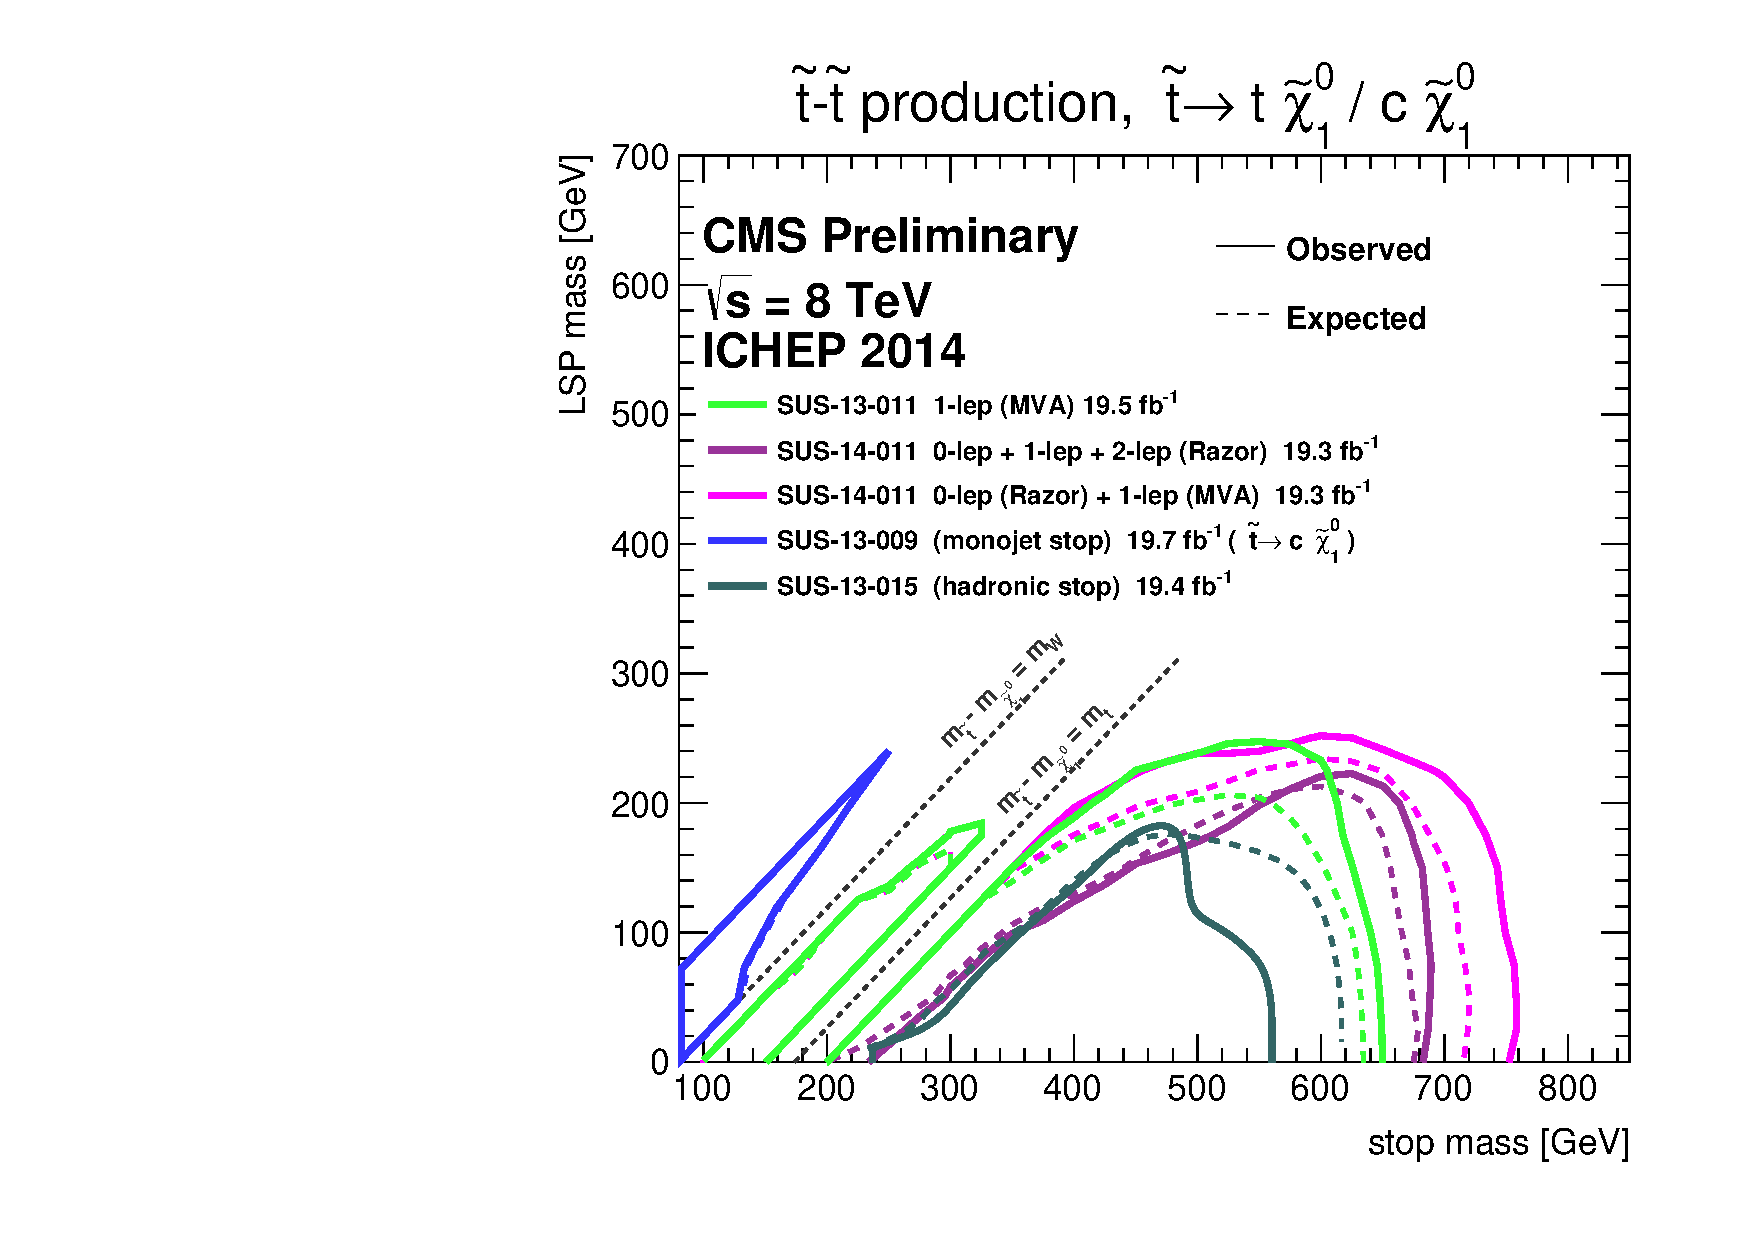
\includegraphics[width=\textwidth]{Figs/other_limits/T2tt_ICHEP2014_All.pdf}
    \caption{CMS}
    \label{fig:cms_current_limit}
  \end{subfigure}\\
  \begin{subfigure}[b]{0.65\textwidth}
    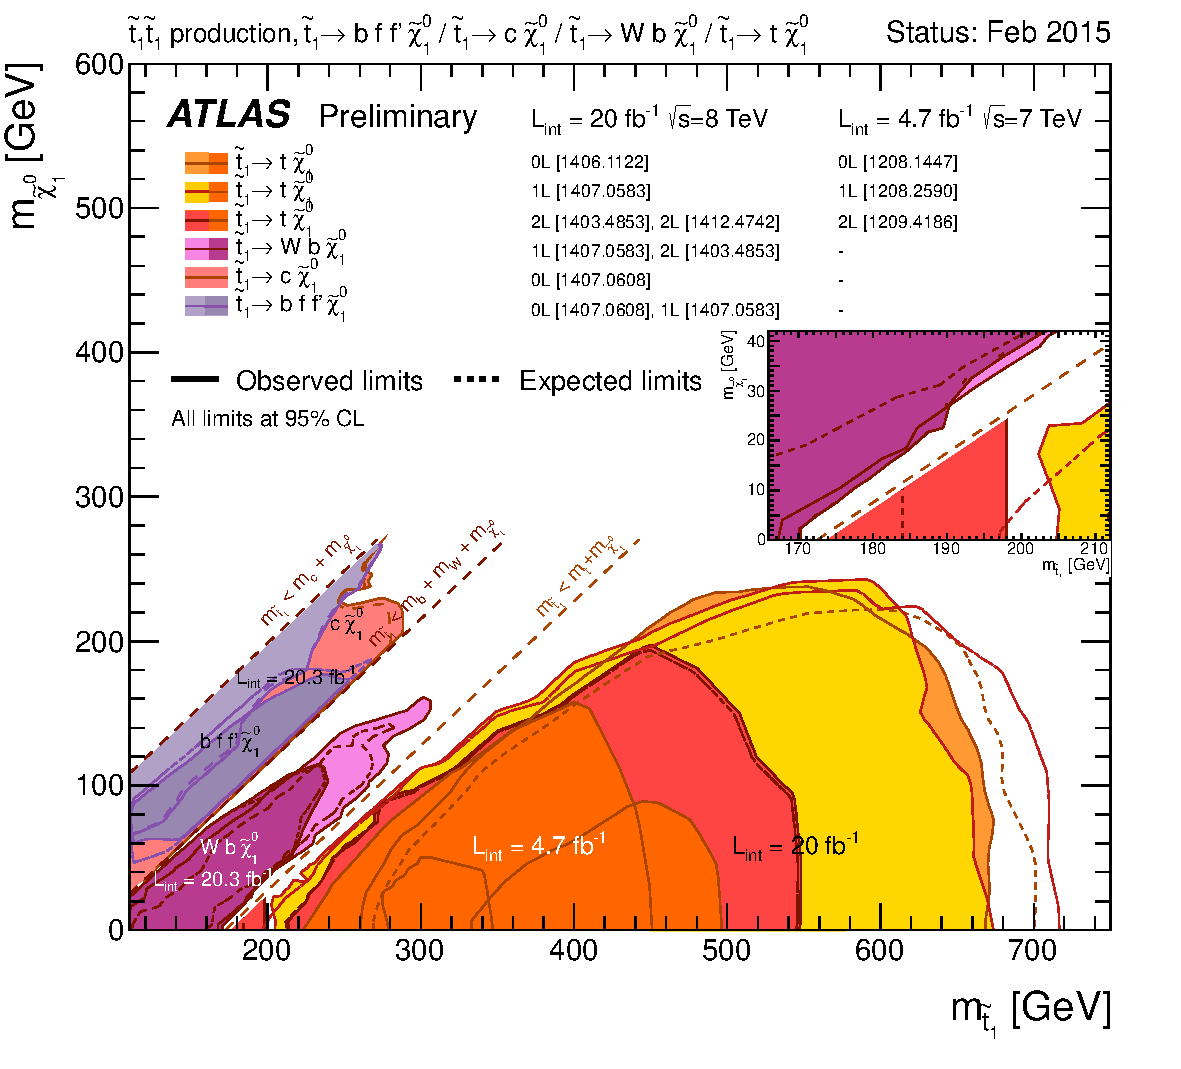
\includegraphics[width=\textwidth]{Figs/other_limits/ATLAS_SUSY_Stop_tLSP.pdf}
    \caption{ATLAS}
    \label{fig:atlas_current_limit}
  \end{subfigure}
  \caption{Current limits on direct stop production from the CMS
  (\ref{fig:cms_current_limit})\cite{cmssusyresults} and ATLAS
  (\ref{fig:atlas_current_limit})\cite{atlassusyresults}
  experiments as a function of the $m_{\sTop} \text{ vs. } m_{\chiz}$ mass
  plane.}
  \label{fig:current_limits}
\end{figure}

Given the current lack of experimental observation, limits for direct \sTop
production are shown in figure~\ref{fig:current_limits}, with observed limits
reaching up to $m_{\sTop} = 275$~\gev for the charm decay, and a similar reach
for the 4-body decay.